
\section{Shorter Questions}

\subsection{What is a ROC curve? How can it be used to evaluate the performance of a
classifier?}
An ROC curve is a graph that displays the True positive rate vs. the False positive rate. 
It is used as a signifier of how well a classifier is performing.
In a classifier it is desirable to have a high true positive rate and a low false positive rate,
as such it is desirable to have a graph that goes straight up to the top left corner and then straight up.
\par 
A useful metric which can be derived from the ROC curve is the area under curve (AUC).
The AUC is a number between 0 and 1 with 1 being a perfect classifier that produces only true positives and no false positives.

\begin{figure}[H]
    \centering
    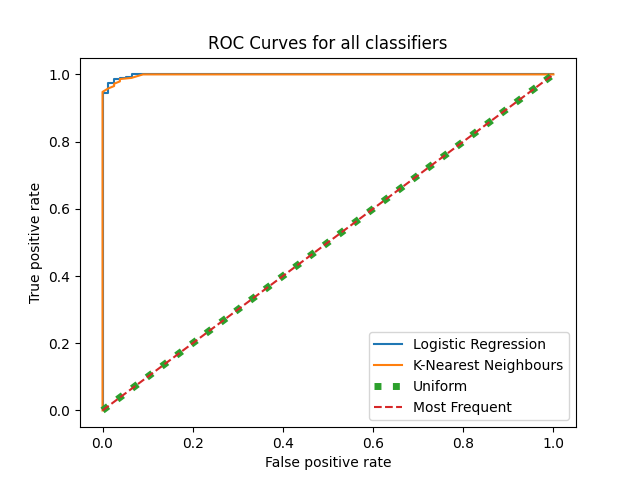
\includegraphics[width=0.5\textwidth]{images/Roc1.png}
    \caption{An old ROC graph that I made for the week 4 assignment.}
    \end{figure}
\par


\subsection{Give two examples of situations when a linear regression would give inaccurate
predictions. Explain your reasoning?}

Linear regression is useful in a number of situations but obviously unsuitable in others.
\par

\textbf{Situation 1: Non-linear data\\}
When the data does not follow a linear trend and this is not accounted for in feature engineering it may not perform adequatly.

This can be prevented by using polynomial combinations of features which better capture the relationships between features.
\par
\textbf{Situation 2: Discreet Value Data\\}
In situations that produce values at discreet intervals (such as the bike prediction above), 
linear regression will almost always be a bit off. 
This data could almost be considered categorical as there are clear, 
discreet possible values of output but this is inapropriate as the values are not all of equal significance and order is important.
This could be counteracted and made more accurrate by rounding the output values.

\subsection{Discuss three pros/cons of an SVM classifier vs a neural net classifier.}


\textbf{Understandability\\}
An SVM is usually easier to understand than most neural nets. 
Each parameter is given a coefficient which makes it easy to see what features are important in the classification/regression problem.
\par
Neural nets are often confusing and treated as black boxes.
It can be difficult to determine how it will react to a particular input. 
\par
\textbf{Training Time\\}
An SVM can be trained far quicker and with a far less powerful computer than a neural net in most cases.
Neural nets can take a very long time to train sometimes depending on the number of parameters and epochs and often need a graphics card to speed up training by doing multiple calculations concurrently.
\par 

\textbf{Performance\\}
Neural Nets are proving to be far better than SVMs and many other methods for a number of problem types.
For example, A convolutional neural bet has acheived an error rate of 0.17\% on the MNIST dataset whereas 
an SVM has only acheived a 0.56\% Error rate.

\subsection{Describe the operation of a convolutional layer in a convNet. Give a small
example to illustrate}
A convolutional layer performs convolutions on a matrix of input features, often an image. 
It does this by moving a sliding window over the image and performing many local convolutions and passing these on to the next layer.
The output of a convolutional layer can also be viewed as an image and is usually smaller.
The output for a given input depends on what operation that the kernel is performing.

\begin{figure}[H]
    \centering
    
\includegraphics[width=0.5\textwidth]{images/Untitled.png}
    \caption{An Illustration of a sliding window on an image.}
    \end{figure}
\par

\subsection{In k-fold cross-validation a dataset is resampled multiple times. What is the
idea behind this resampling i.e. why does resampling allow us to evaluate the
generalisation performance of a machine learning model. Give a small example
to illustrate.}
Resampling is done so that all parts of the data are used for both training and validation at different times.
The data is randomly split into k 'folds'. 
A model is trained on k-1 of these folds and then tested on that final fold.
This is done multiple times until each fold is used to test.
This allows us to get an idea of the performance of the model on the entire dataset and not just part of it.


